\section{Kort introduktion till programmering i \coq{} och utvecklingsmiljön
\coq{} Ide}

\subsection{Beskrivning av \coq{} Ide}


\coq Ide är en interaktiv utvecklingsmiljö där användaren kan
formulera bevis och skriva program och få hjälp med att bevisa
dessa. I följande avsnitt förklaras de viktigaste delarna med
hjälp av skärmdumpar från olika exempel.


Figur~\ref{fig:oversikt} är en översikt av hela utvecklingsmiljön och dess olika delar
\begin{enumerate}
\item Textredigerare. I den här rutan skriver användaren sina program och bevis
\item Textfönster för mål och kontext. Här visas vilka mål man vill uppnå och
  vilka värden man för närvarande har i kontext. Dessa uppdateras efter varje
  utförd taktik.
\item Textfönster för meddelanden. Här dyker felmeddelanden, svar på
  gjorda sökningar och övrig information upp.
\item Symboler för att stega framåt eller bakåt i koden. När vi stegar framåt
  evalueras koden som stegas förbi.
\end{enumerate}

\filbreak

\begin{figure}[H]
  \centering
  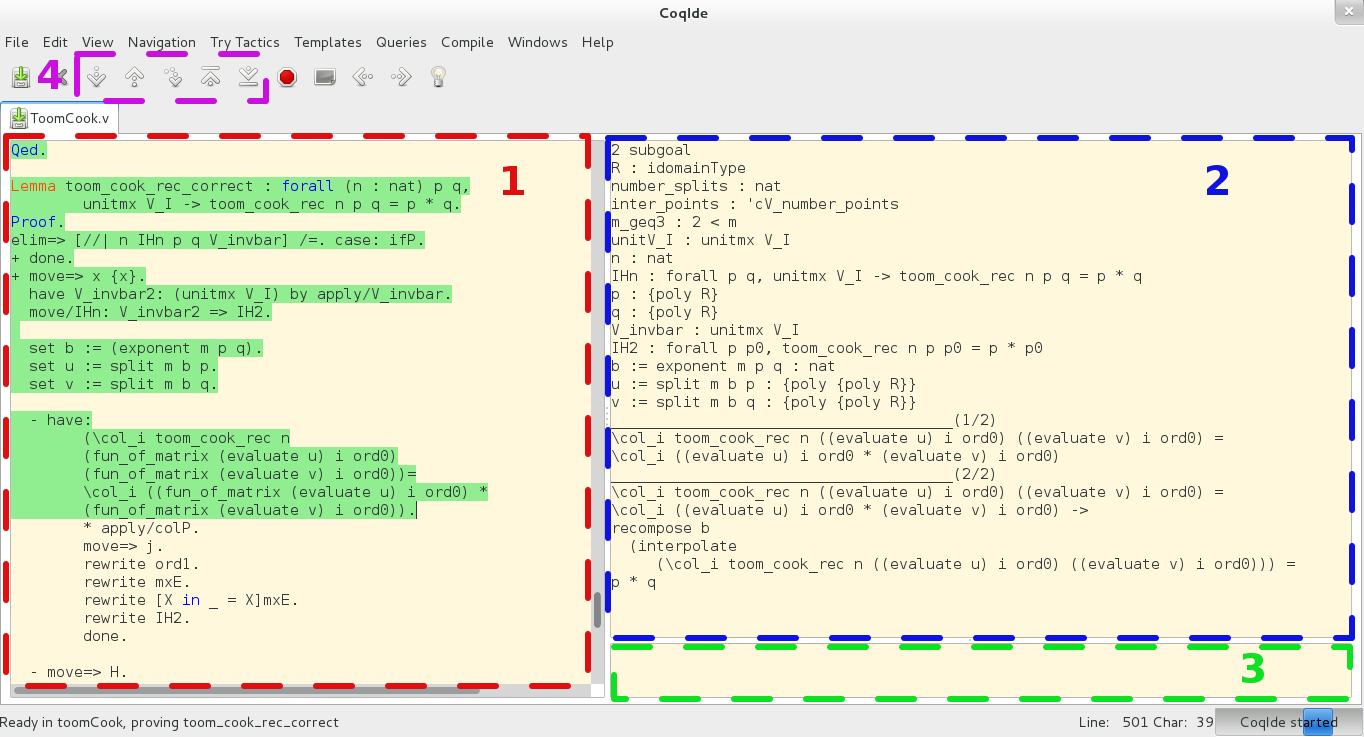
\includegraphics[width=\textwidth]{images/Overview}
  \caption[Översikt av \coq{} Ide]
   {Översikt av de olika delarna i \coq{} Ide}
  \label{fig:oversikt}
\end{figure}

Figur~\ref{fig:kontext} är är en förstoring av ruta 2 i Figur~\ref{fig:oversikt}
\begin{enumerate}
  \setcounter{enumi}{4}
\item Kontext, här visas vilka hypoteser och variabler som vi för tillfället
  har i beviset.
\item Mål, här visas vilka mål som ska uppnås. Det översta målet är det som
  användaren arbetar med för tillfället och det är det målet som kommer att
  påverkas av nästkommande taktik.
\end{enumerate}

\begin{figure}[H]
  \centering
  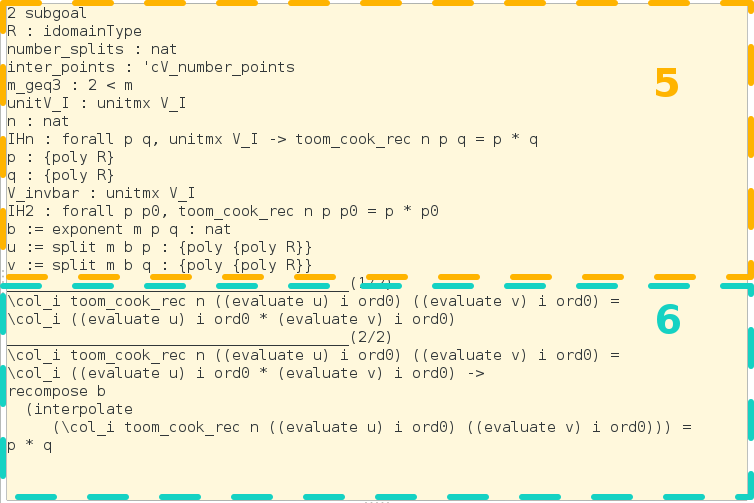
\includegraphics[width=150mm]{images/Kontext}
  \label{fig:kontext}
  \caption[Fönster för kontext och mål]
   {Textfönster för kontext och mål. Figuren visar en förstoring av ruta 2 i
    figur 4.1}
\end{figure}




\subsection{Evaluering av kod}
\coq{} är uppbyggt av satser där varje sats avslutas med en punkt. Koden
evalueras sedan en sats i taget och de delar av koden som har blivit evaluerade
markeras med en grön färg och det går inte längre att göra några ändringar i
dessa. Om man skulle vilja göra en ändring får man stega tillbaka
i programmet och göra ändringen. I följande sekvens av skärmdumpar visas
hur ett bevis

Figur~\ref{fig:bevis1} visar ett exempel på ett bevis för att följande påstående
är en tautologi. En tautologi är en logisk sats som alltid är sant oberoende av
sanningsvärdena på hypoteserna.


\begin{figure}[H]
  \centering
  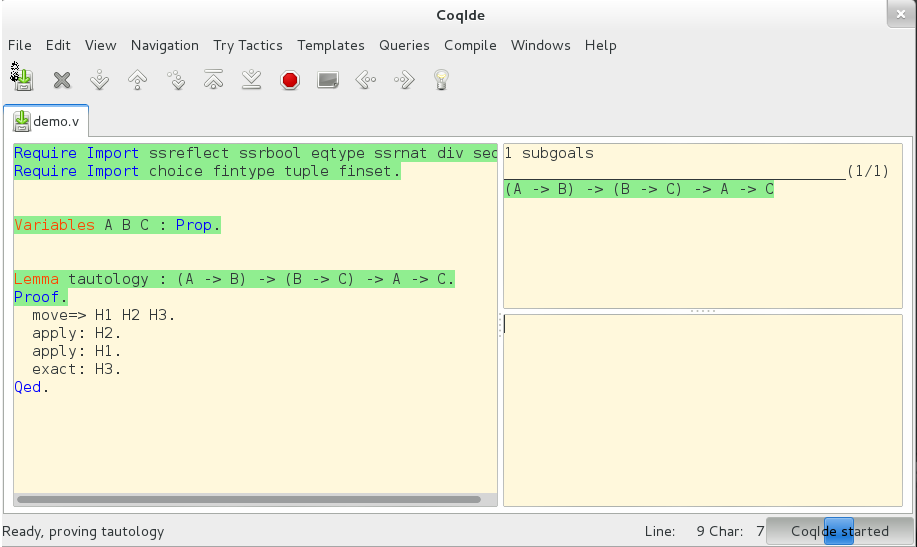
\includegraphics[width=100mm]{images/Proof_part1}
  \label{fig:bevis1}
  \caption[Exempel på bevis i \coq{}]
   {Exempel på ett bevis för en tautologi i \coq{}}
\end{figure}

Figurerna ~\ref{fig:bevis2} och ~\ref{fig:bevis3} visar den interaktiva
biten mellan \coq Ide och användaren. Notera hur mål och kontext uppdateras
efter att en taktik används och attden taktik som har evaluerats blir grönmarkerad.


\begin{figure}[H]
  \centering
  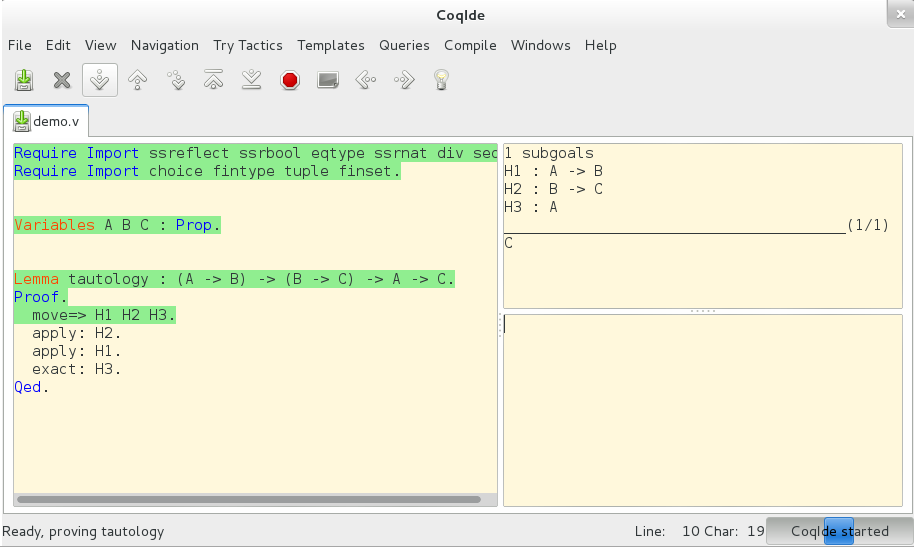
\includegraphics[width=150mm]{images/Proof_part2}
  \label{fig:bevis2}
  \caption[Bevis i \coq{} Ide]
   {Vi har nu flyttat hypoteserna (A $rightarrow$ B), (B $\rightarrow$ C) och A
    från målet till kontexten och med taktiken \C{move}}
\end{figure}

\begin{figure}[H]
  \centering
  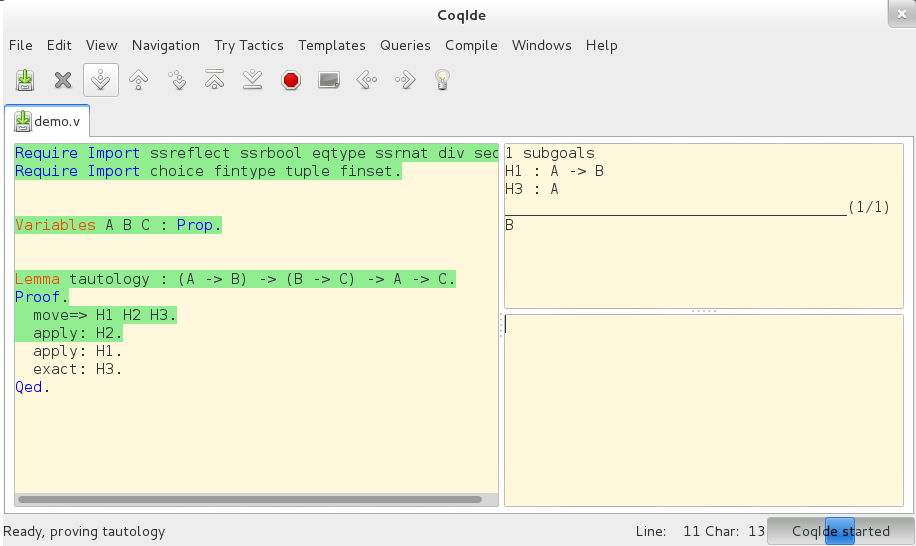
\includegraphics[width=150mm]{images/Proof_part3}
  \label{fig:bevis3}
  \caption[Bevis i \coq{} Ide]
   {Vi har nu använt oss av Hypotesen ($B \rightarrow C$) och vi
    kan se att målet nu har ändrat sig från C till B}
\end{figure}
